\section{Initial Ideas}
The initial approach to the magnetism task focused on reliably detecting the static magnetic fields emitted by the ducks to identify species through their distinct polarities. Early testing with the DRV5053 Hall sensor revealed significant challenges in achieving consistent detection. When the sensor was placed in direct contact with the duck's head, the output voltages correctly indicated the magnetic polarity. However, at even small distances of just a few millimetres, the signal strength dropped dramatically, making it impossible to determine the field direction reliably.

These preliminary results made it clear that additional signal conditioning would be necessary for practical implementation. The key requirements emerged as amplifying the weak magnetic signals to extend the detection range while implementing proper filtering to stabilize the output against noise. The trade-offs between sensitivity, noise immunity, and physical positioning became the primary focus for further development.

\section{Hall Effect Sensor}
The Hall effect sensor operates on the principle of detecting magnetic fields through the deflection of charge carriers in a semiconductor material. When exposed to a magnetic field perpendicular to its sensing surface, the sensor generates a voltage proportional to the field strength. Our initial testing with the DRV5053 sensor revealed several important characteristics about its behaviour in our specific application. With the sensor placed directly against the duck's head, the output voltage clearly indicated the magnetic polarity. However, this reliable detection only occurred at impractically close distances.

\section{DRV5053 Hall Sensor Analysis}
\begin{table}[H]
    \centering
    \begin{tabular}{|p{4cm}|p{10cm}|}
        \hline
        \textbf{Sensor Characteristic} & \textbf{Analysis}                                                                                                                                                                                                                                                                                                                     \\
        \hline
        Field and Polarity Detection   & Detects static magnetic fields from the ducks; distinguishes magnetic fields based on voltage increases/decreases from the 1.0V baseline. Sensor response is maximized when the magnetic field is aligned perpendicular to the sensor face, adhering to the Lorentz force principle (\( F = B \cdot I \cdot L \cdot \sin(\theta) \)). \\
        \hline
        Output Type                    & Linear voltage (0.2V to 1.8V) centred around 1.0V with no magnetic field.                                                                                                                                                                                                                                                             \\
        \hline
        Temperature Stability          & Maintains ±10\% sensitivity over –40°C to 125°C - stable for varying environments.                                                                                                                                                                                                                                                    \\
        \hline
        Noise Level                    & As low as 5mV\textsubscript{pp} but filtering may be required to ensure signals are stable under weaker magnetic fields.                                                                                                                                                                                                              \\
        \hline
    \end{tabular}
    \caption{DRV5053 Hall Sensor Characteristics}
    \label{tab:sensor_characteristics}
\end{table}

The LTspice ideal model of the DRV5053 (Figure 7.1) produced a clean and stable output waveform when modelled with ideal conditions, showing distinct voltage levels for north and south pole detection. The simulated output of the DRV5053 LTspice model (see Figure 7.2) perfectly matched our microcontroller's analogue input specifications with its 0.2V to 1.8V output range. However, testing exposed several significant limitations that needed addressing. The most critical issue became apparent when attempting to detect fields at even modest distances of just a few centimetres – the output signal weakened dramatically, making reliable polarity detection impossible. The sensor's sensitivity proved insufficient for our required detection range, as the magnetic field strength diminished rapidly with distance according to the inverse-square law.
\begin{figure}[H]
    \centering
    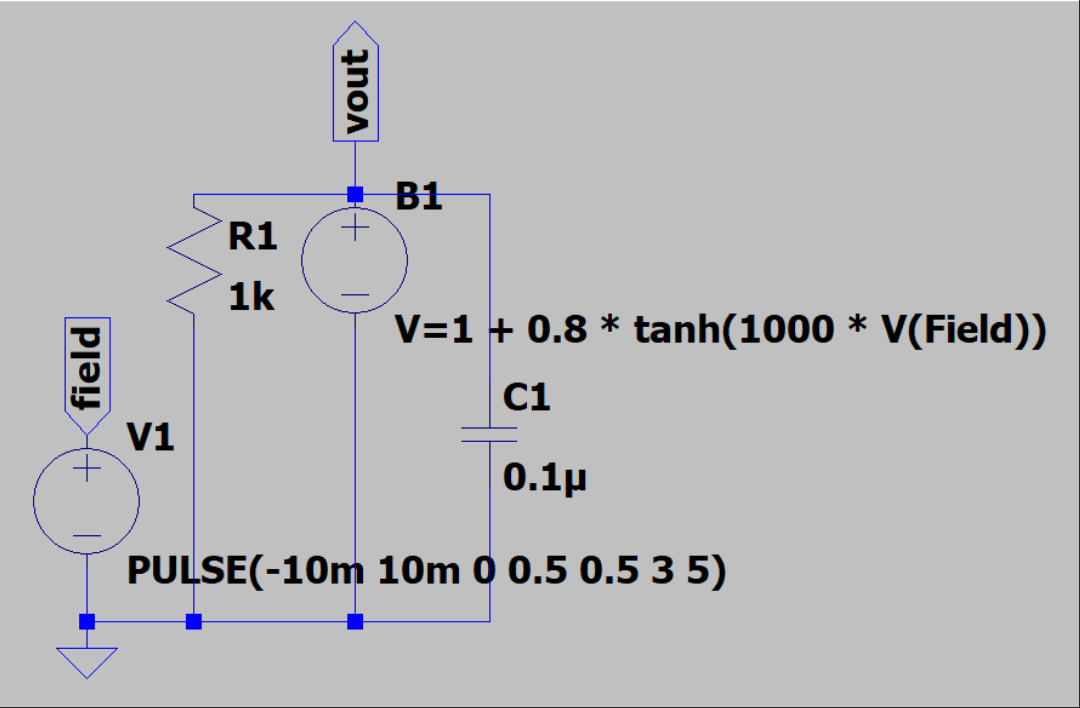
\includegraphics[width=0.6\textwidth]{subpages/images/magnet_model.png}
    \caption{LTspice Ideal Model of DRV5053}
    \label{fig:ideal_model}
\end{figure}
\begin{figure}[H]
    \centering
    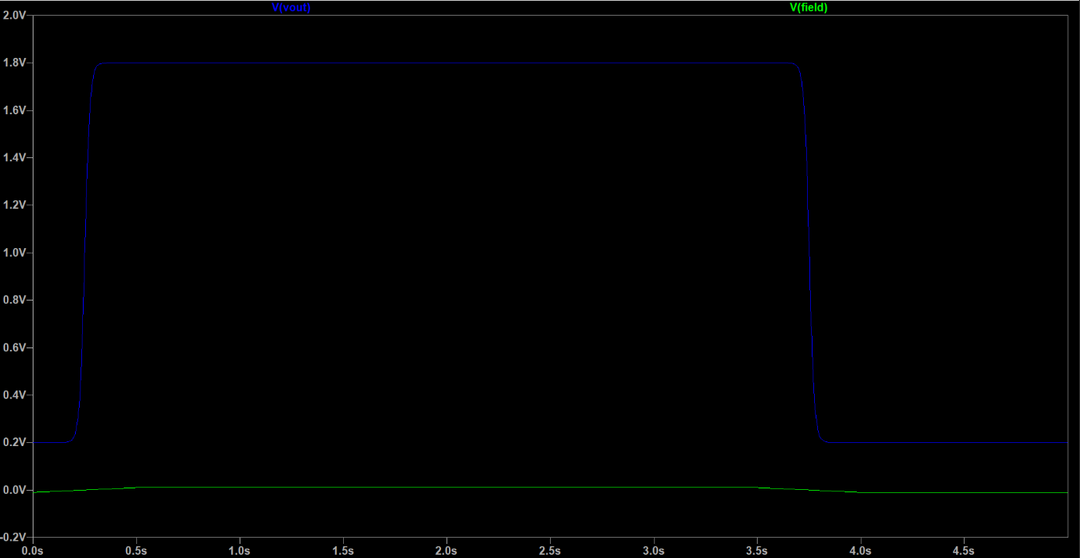
\includegraphics[width=0.6\textwidth]{subpages/images/magnet_out.png}
    \caption{Output of DRV5053 LTspice Model}
    \label{fig:model_output}
\end{figure}
These findings made it clear that additional signal conditioning would be necessary for reliable operation. The output required amplification to boost the detectable range.


\section{Amplification}
\begin{figure}[H]
    \centering
    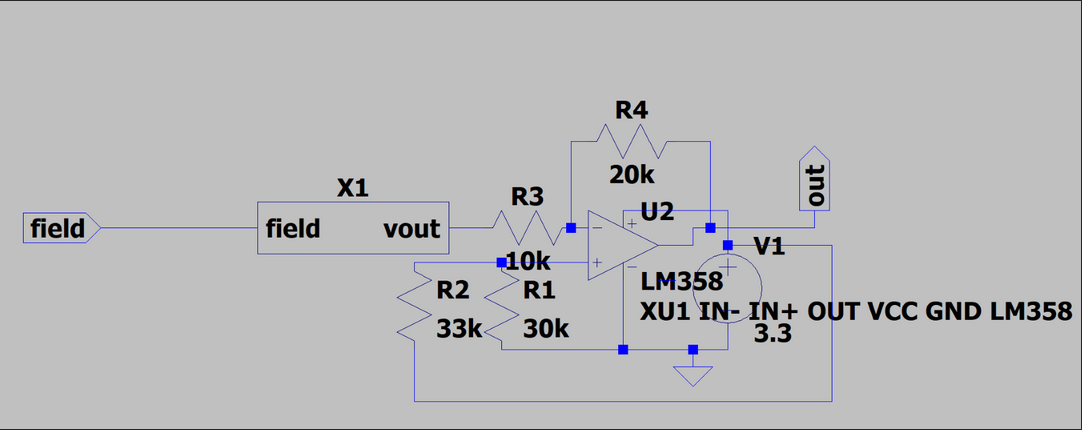
\includegraphics[width=0.6\textwidth]{subpages/images/magnet_circuit.png}
    \caption{Final Circuit Diagram}
    \label{fig:circuit}
\end{figure}
The amplification stage plays a critical role in ensuring reliable detection of the duck's magnetic field. The LM358 operational amplifier, configured as an inverting amplifier with a gain of -10, is illustrated in Figure 7.3. It uses a 10kΩ input resistor and 100kΩ feedback resistor to boost the Hall sensor's weak 0.2V-1.8V output to a more usable 0V-3.3V range compatible with the Metro M0's ADC inputs. The circuit includes a 1.1V virtual ground reference to enable proper single-supply operation by effectively creating a mid-supply point for the op-amp's inputs and outputs. Careful design ensures the amplified signal remains within the 0V-3.3V range, significantly improving the system's ability to detect and classify ducks at distances up to 6.5cm - a huge improvement over the raw Hall sensor output.
\begin{table}[H]
    \centering
    \begin{tabular}{|c|c|c|}
        \hline
        \textbf{Offset (V)} & \textbf{Gain (mV)} & \textbf{Distance (cm)} \\
        \hline
        1.1                 & -4.7               & 3.5                    \\
        \hline
        1.1                 & -6.8               & 4.5                    \\
        \hline
        1.1                 & -10                & 6.5                    \\
        \hline
    \end{tabular}
    \caption{Hall Sensor Output vs Distance}
    \label{tab:hall_output_distance}
\end{table}

\section{Building and Testing}
The final assembled circuit for the Hall sensor and amplification stage is shown in Figure 7.4.

Comparing these experimental results with the ideal LTspice simulations (Figures 7.1 and 7.2), it's evident that while the simulations provided a theoretical understanding of the sensor's behaviour, real-world conditions presented additional challenges. They did not account for the rapid signal attenuation over distance that was observed in physical testing.
\begin{figure}[H]
    \centering
    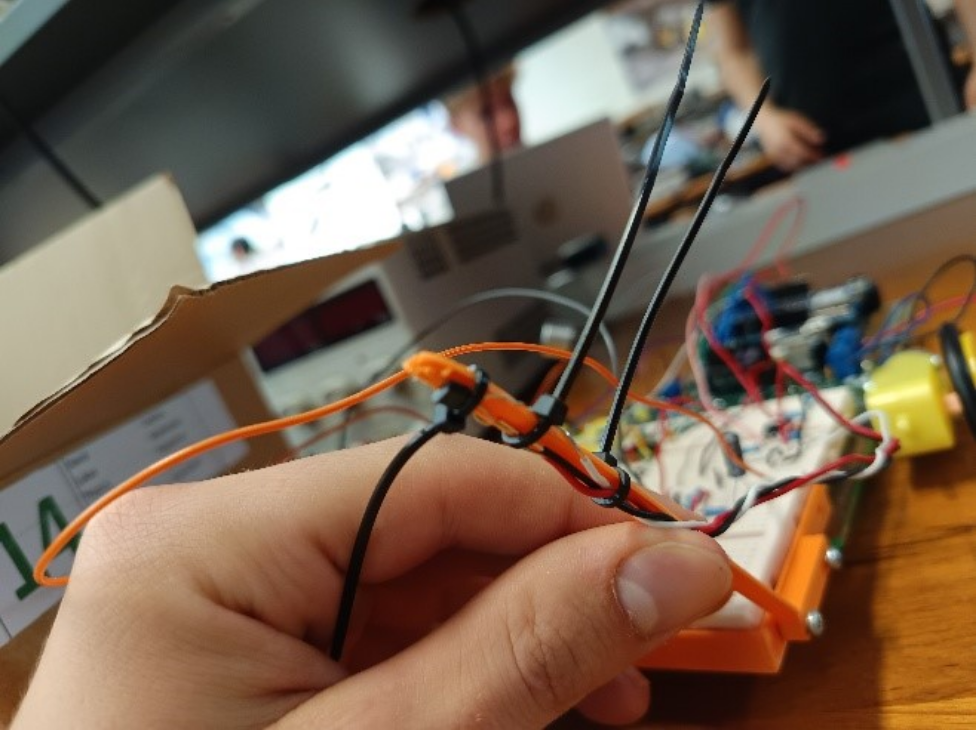
\includegraphics[width=0.7\textwidth]{subpages/images/magnet_arm_irl.png}
    \caption{Arm for Hall Sensor}
    \label{fig:magnet_arm}
\end{figure}
\begin{figure}[H]
    \centering
    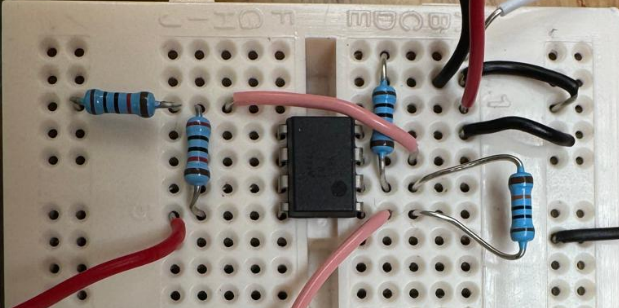
\includegraphics[width=0.7\textwidth]{subpages/images/magnet_circuit_irl.png}
    \caption{Final Circuit}
    \label{fig:circuit_irl}
\end{figure}
Since the magnet is placed facing up inside the duck’s head, the sensor needs to face the top of the duck’s head to detect the magnetic field. To implement this, we 3D printed an arm for the sensor to position it over the duck.

The need for amplification, as demonstrated by the improved detection distances in the table, was a direct consequence of these real-world limitations, highlighting the gap between ideal simulation and practical implementation. While the ideal model showed a clean signal, the physical setup necessitated amplification to achieve robust performance, especially at weaker magnetic fields. The discrepancy between simulated ideal conditions and physical testing underscores the importance of iterative design and validation, where simulations provide a baseline, and practical experiments reveal critical design requirements like amplification.